\chapter{Reglerentwurf} \label{ch_Reglerentwurf}
In diesem Kapitel werden die Eigenschaften des zu regelnden Modells vorgestellt und darauf aufbauend dessen Ein- und Ausgangsgrößen festgelegt.
Anschließend wird ein geeigneter Regler vorgestellt und der resultierende Regelkreis abgeleitet.
Zuletzt wird die Übertragbarkeit der Regelung auf das Realsystem des Solarturmkraftwerkes in Jülich untersucht.

\section{Systemeigenschaften} \label{sec_Systemeigenschaften}
Die in Kapitel \ref{ch_Modellbildung} vorgestellte Modellierung des Solarturms bildet sowohl den Einfluss der 2153 Heliostaten als auch den des Luftstroms im Receiver ab.
An der Innenseite des Receivers tritt einzig die aufgeheizte Luft aus und steht dem nachfolgenden Prozess zur Verfügung.
Daher gehört das System zu den sogenannten \mbox{\textit{MISO}-Systemen} (\textbf{M}ulti \textbf{I}nput \textbf{S}ingle \textbf{O}utput), mit mehreren Eingangs- und einer Ausgangsvariablen.

Das Modell zeichnet sich durch die Inbezugnahme zeitabhängiger Parameter aus.
Die modellierte Einstrahlung auf das Heliostatenfeld wird mithilfe einer Wolkensimulation beeinflusst.
Auf diese Weise ergibt sich ein dynamisches System bei dem die Ausgangsgröße nicht ausschließlich von den Regelungsgrößen abhängig ist.


\subsection{Wahl der Stell- und Regelgrößen} \label{subsec_EinAusgangsgrößen}
In der vorliegenden, rein simulativen Betrachtung ergeben sich die Stellgrößen direkt aus den Eingangsgrößen des in Kapitel \ref{ch_Modellbildung} vorgestellten Modells, da die explizite Betrachtung von Stellgliedern wie den Motoren der Heliostaten entfällt.
Somit sind die Stellgrößen:
\begin{itemize}
    \item Die drei Streuungsfaktoren $\kappa_1$, $\kappa_2$ und $\kappa_3$ zur Beeinflussung der Heliostatpositionen
    \item Der Einstellwert $u_{\mathrm{Setpoint}}$ der Gebläse-/Ventil-Kombination im Receiver
\end{itemize}
Die solare Einstrahlung dient dem Modell zwar als Eingangsgröße, wird jedoch nicht vom Regler beeinflusst und stellt daher keine Stellgröße dar.

Der Enthalpiestrom $\dot{H}_{\mathrm{out}}$ am Auslass des sekundären Headers (vgl. Kapitel \ref{subsubsec_Header} und Abbildung \ref{fig_ZusammenfassungKopplung}) kennzeichnet die einzige Ausgangsgröße des Modells und somit auch die Regelgröße.
Dies ist sinnvoll, da die Temperatur des austretenden Luftmassenstroms direkten Einfluss auf den Wirkungsgrad der Anlage hat, dessen Maximierung Ziel dieser Arbeit ist.

\subsection{Analyse der Systemdynamik} \label{subsec_Systemdynamik}
In Abbildung \ref{fig_Sprungantwort} ist die Dynamik des Systems in Form der Sprungantwort bei Änderung der Einstrahlung dargestellt.
Im untersten Teil der Grafik ist erkennbar, dass der Einstellwert des Lüfters und damit der Luftmassenstrom im Receiver konstant gehalten wird.
Ebenfalls konstant sind die Streuungsfaktoren (zweiter Graph von unten), jedoch sinkt die solare Einstrahlung auf den Receiver nach $100$ Sekunden von $\SI{100}{\percent}$ auf $\SI{25}{\percent}$ ab (oberer Graph).
Dies hat zur Folge, dass, wie im mittleren Graphen zu sehen, die vom Receiver absorbierte Leistung und die Maximaleinstrahlung auf einen einzelnen Cup um $\SI{75}{\percent}$ abfallen.
Dadurch sinkt die Temperatur an der Absorber-Front (zweiter Graph von oben) und die Luftaustrittstemperatur im Receiver (oberer Graph).
Die Angaben zu den Grenzen der Fronttemperatur sowie dem Sollwert der Austrittstemperatur werden in Kapitel \ref{subsec_ParameterMPC} erläutert.

\begin{figure}[h!]
    \centering
    \setlength{\fboxsep}{1pt}
    \setlength{\fboxrule}{1pt}
    \fbox{\includegraphics[width=0.99\textwidth]{C:/Users/gesc_ma/VSCode MPC Projekt/dynaovrcontroller/dynaovrcontroller/aimpoint_control_scenarios/plots/00_no_control/100_to_25.png}}
    \caption[Sprungantwort des Modells im offenen Regelkreis bei Veränderung der solaren Einstrahlung von $\SI{100}{\percent}$ auf $\SI{25}{\percent}$]{Sprungantwort des Modells im offenen Regelkreis bei Veränderung der solaren Einstrahlung von $\SI{100}{\percent}$ auf $\SI{25}{\percent}$}
    \label{fig_Sprungantwort}
\end{figure}

Die sogenannte Ausregelzeit zeigt, wie lange die Dauer zwischen dem Gleichgewichtszustand vor und nach der Anregung ist.
Dabei wird nach \cite[S.223]{Zacher} eine Toleranz von $\SI{4}{\percent}$ angesetzt, um den Zeitpunkt zu ermitteln, bei dem der resultierende Gleichgewichtszustand erreicht wird.
An der Temperatur der Austrittsluft in Abbildung \ref{fig_Sprungantwort} ist erkennbar, dass die Ausregelzeit des Modells bei $T_{\mathrm{settling}} = \SI{450}{\second}$ liegt.

\section{Eigenschaften des Reglers} \label{sec_Reglereigenschaften}
Zur effektiven Regelung des Modells wird nachfolgend ein geeigneter Reglertyp ausgewählt und parametrisiert.
Ergebnisse der Regelung werden in Kapitel \ref{ch_AnalyseRegelung} diskutiert.


\subsection{Wahl des Regelverfahrens} \label{subsec_ReglerverfahrenWahl}
Im Anwendungsfall dieser Arbeit sind bezüglich der geeigneten Regelung die folgenden Kriterien relevant:
\begin{itemize}
    \item Zukünftige Modellparameter müssen prädiktiv in die Regelung einbezogen werden können,
    \item die Regelung von MISO-Systemen soll unter ohne Untergliederung in kleinere Teilsysteme geschehen können,
    \item Limitierungen auf die Ein- und Ausgangsgrößen des Systems müssen implementierbar sein.
\end{itemize}
Klassische Regler wie der PID- oder LQR-Regler, die lediglich auf Basis der Abweichung von aktuellen Soll- und Istwerten Stellgrößen für das System vorgeben \cite[S.408]{Lunze} eignen sich daher nicht für die vorgesehene Regelung des Solarturms.
Wie in Kapitel \ref{subsec_GrundlagenMPC} dargestellt, eignet sich eine modellprädiktive Regelung für das dargestellte Anforderungsprofil.


\subsection{Parametrisierung des MPC} \label{subsec_ParameterMPC}
Neben der für jede Art von Regelung relevanten Abtastzeit (\textit{Sample Time}) $T_s$, also der Zeit zwischen zwei Berechnungsschritten, werden nachfolgend die MPC-spezifischen Regelparameter bestimmt.
Dazu gehören, wie in Kapitel \ref{subsec_GrundlagenMPC} ersichtlich, der Prädiktionshorizont $N_2$ sowie der untere und obere Regelungshorizont $N_1$ bzw. $N_u$.
Weiterhin werden die Constraints, also die Parameterlimitierungen, eingeführt und die Kostenfunkton der Regelung bestimmt.

\subsubsection*{Abtastzeit} \label{subsubsec_sampletime}
Die Abtastzeit wird durch eine untere und eine obere Grenze limtiert.
Die untere Grenze ergibt sich daraus, dass das System als quasistatisch angesehen wird (vgl. Kapitel \ref{subsec_ModifikationAlgorithmus}).
Daher muss zwischen zwei Berechnungsschritten genug Zeit vergehen, dass der Regler die optimalen Streuungsfaktoren errechnen kann und die Heliostaten den nächsten Zielpunkt auf dem Receiver erreichen können.
In \cite[S.25-26]{DissZanger} ist die Dynamik der Heliostaten in Jülich dargestellt.
Bei Vernachlässigung der Rechenzeit ergibt sich die minimale Abtastzeit zu $\SI{2.79}{\second}$.

Die obere Grenze ist davon abhängig, nach welcher Zeit eine erhöhte Flussdichte auf dem Receiver diesen beschädigt.
Dabei entsteht die Schädigung des Receivers nicht durch die erhöhte Einstrahlung an sich, sondern durch die Überschreitung der thermischen Spannungen durch die erhöhte Fronttemperatur.
Daher muss die Abtastzeit kleiner sein, als die Zeit, in der eine erhöhte Flussdichte kritische Spannungen erzeugt.

Im schlechtesten Fall tritt die Überschreitung der Flussdichte unmittelbar nach dem vorigen Berechnungsschritt auf, sodass diese Information erst beim nächsten Abtastzeitpunkt zur Verfügung steht und der Regler erst in der darauf folgenden Berechnung reagieren kann.
Folglich benötigt der Regler zwei Abtastzeitpunkte um auf eine überhöhte Einstrahlung reagieren zu können.
Daher darf die maximale Abtastzeit bei der Hälfte einer kritischen Zeit $t_{\mathrm{max}}$ liegen, in der eine erhöhte Flussdichte den Receiver beschädigt.

Die kritische Zeit $t_{\mathrm{max}}$ wird in dieser Arbeit als die Zeit definiert, in der eine um $\SI{10}{\percent}$ höhere Flussdichte als vom Regler erwartet einen Anstieg der Fronttemperatur von $\SI{20}{\kelvin}$ verursacht.
In Abbildung \ref{fig_SampleTimebestimmen} ist ein solches Szenario ohne Regeleingriff dargestellt.
Es ist ersichtlich, dass die Fronttemperatur des Receivers bereits innerhalb von $t_{\mathrm{max}} = \SI{56}{\second}$ nach Anstieg der Einstrahlung um $\SI{20}{\kelvin}$ zunimmt.
Daher ergibt sich die maximale Abtastzeit nach Gleichung \ref{eq_SampleTimeberechnen} zu $\SI{28}{\second}$.
\begin{equation} \label{eq_SampleTimeberechnen}
    T_{s, \mathrm{max}} = \frac{t_{\mathrm{max}}}{2}
\end{equation}
% \centerline{\small{\textsf{\textbf{Formel \ref{eq_Label}:}} Beschriftung}}
\myequations{\quad Berechnung der Abtastzeit aus der kritischen Zeit zur Beschädigung des Receivers}

\begin{figure}[h!]
    \centering
    \setlength{\fboxsep}{1pt}
    \setlength{\fboxrule}{1pt}
    \fbox{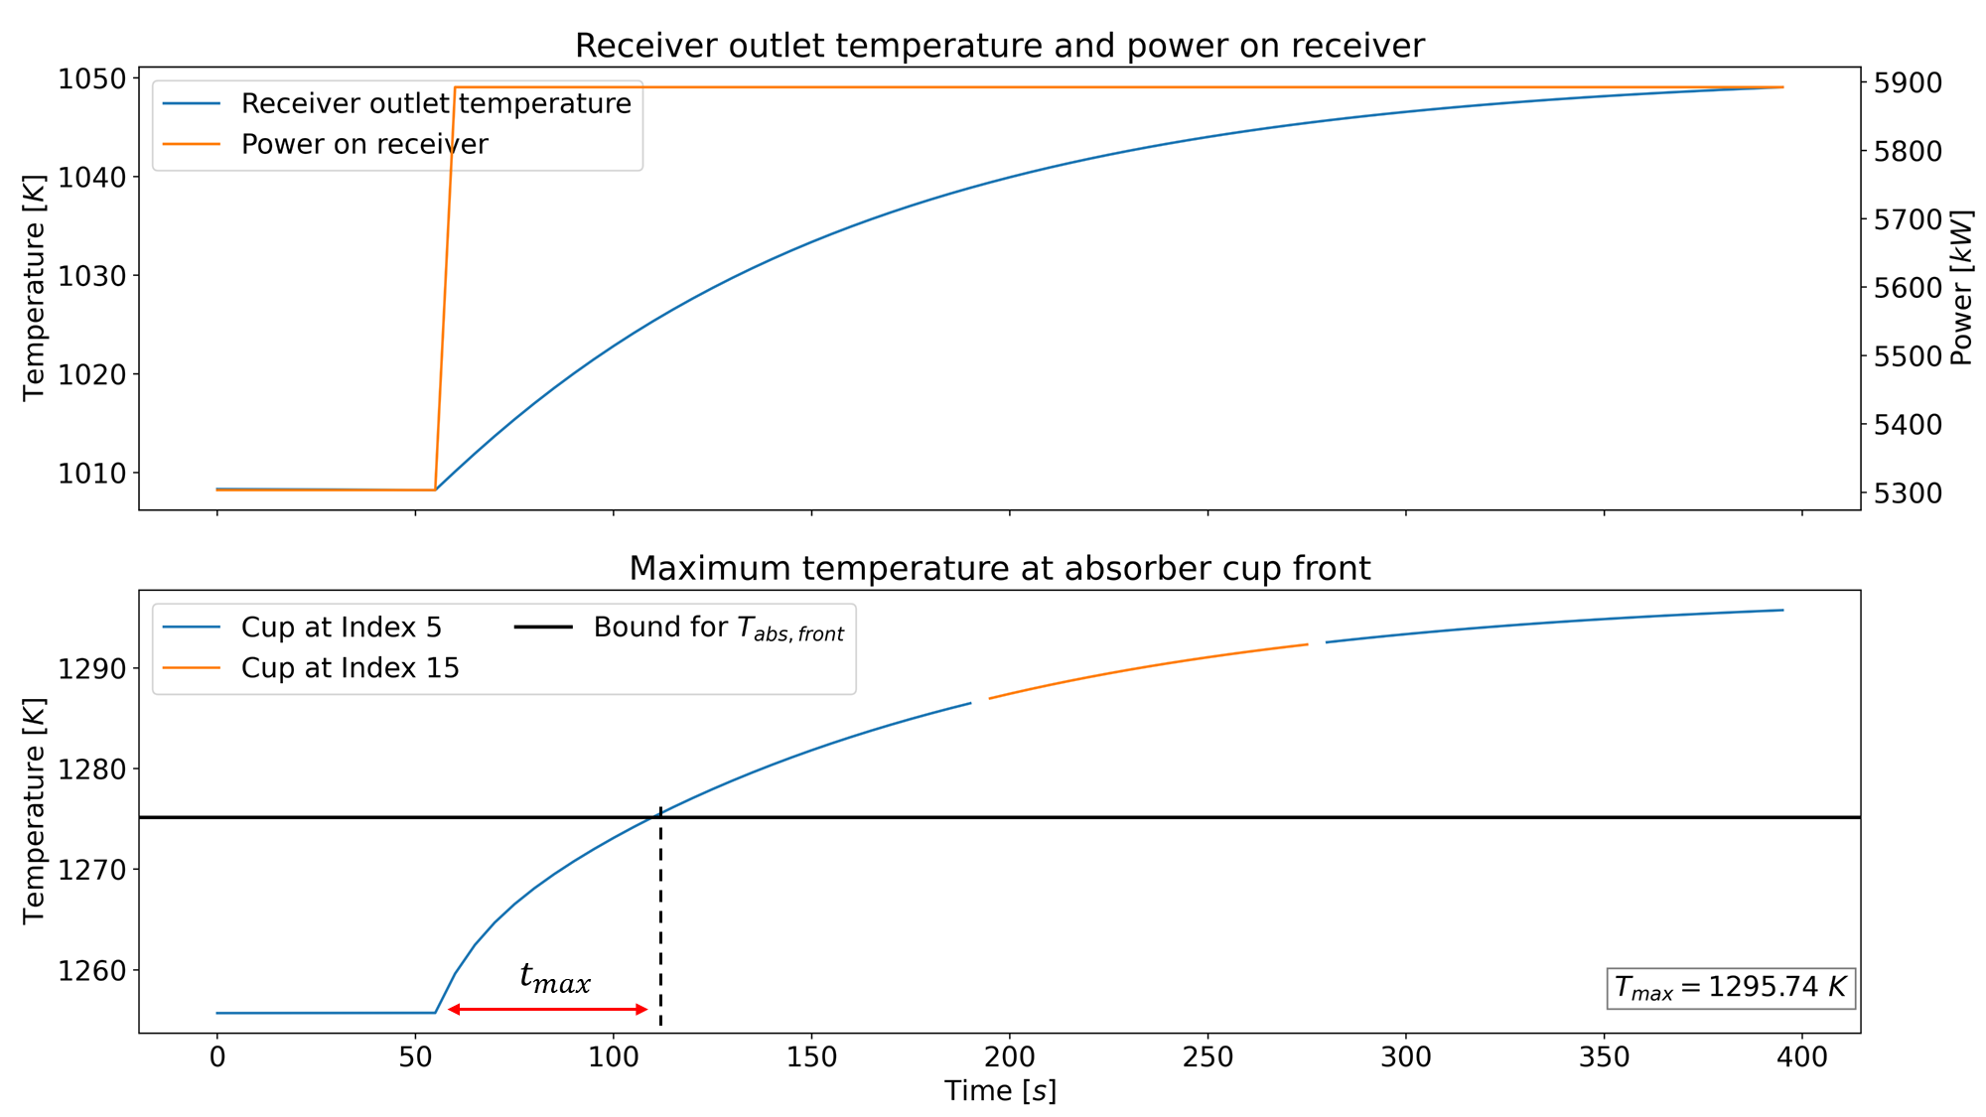
\includegraphics[width=0.99\textwidth]{C:/Users/gesc_ma/VSCode MPC Projekt/dynaovrcontroller/dynaovrcontroller/aimpoint_control_scenarios/plots/00_no_control/10prc_overflux_Temperatures_only_labeld.png}}
    \caption[Simulative Bestimmung der kritischen Zeit $t_{\mathrm{max}}$ bis zur Erhöhung der Receiver-Fronttemperatur um $\SI{10}{\kelvin}$]{Simulative Bestimmung der kritischen Zeit $t_{\mathrm{max}}$ bis zur Erhöhung der Receiver-Fronttemperatur um $\SI{20}{\kelvin}$}
    \label{fig_SampleTimebestimmen}
\end{figure}

Nach empirischer Analyse von Simulationen mit unterschiedlichen Abtastzeiten wird eine Abtastzeit von $T_s=\SI{10}{\second}$ gewählt.
Dies stellt einen guten Kompromiss zwischen einem zu hohen Berechnungsaufwand aufgrund kleiner Abtastzeiten und langsamer Reaktion des Reglers aufgrund zu großer Abtastzeiten dar.


\subsubsection*{Prädiktions- und Regelungshorizont} \label{subsubsec_horizonte}
Für Dauer des Prädiktionshorizontes ist nach \cite{XXX} in erster Iteration die Ausregelzeit zu betrachten.
Auf diese Weise steht dem Regler zur Optimierung die gesamte Systemdynamik von der Anregung bis zum folgenden Gleichgewichtszustand zur Verfügung.
Daran angepasst kann der Kontrollhorizont bestimmt werden.
Dieser sollte $\SIrange{10}{20}{\percent}$ des Prädiktionshorizontes abdecken.

Gemäß Kapitel \ref{subsec_Systemdynamik} wird der Prädiktionshorizont zunächst mit $T_{\mathrm{settling}} = N_{2,\mathrm{initial}} = \SI{450}{\second}$ angenommen.
Auf dieser Basis ergibt sich der obere Kontrollhorizont zu $N_u = 0.15\cdot N_{2,\mathrm{initial}} = \SI{60}{\second}$.
Für den unteren Kontrollhorizont gilt $N_1 = 0$, sodass bereits in erster Iteration des Reglers die Stellgrößen verändert werden und eine schnelle Regelung erfolgen kann.
Da das Ziel der Arbeit die effektive Regelung bei kurzfristiger Änderung der solaren Einstrahlung darstellt, ist die Berechnung der Prädiktionen über einen Horizont von $\SI{7.5}{\minute}$ allerdings sehr hoch.
Um den Berechnungsaufwand zu verringern wird der Prädiktionshorizont dem Regelungshorizont angeglichen.
Daher gilt $N_2 = N_u = \SI{60}{\second}$.

\subsubsection*{Constraints} \label{subsubsec_constraints}
Der Einstellwert des Gebläses als Eingangswert des Modells ist gemäß Betriebshandbuch des Solarturms in Jülich so zu wählen, dass der Luftmassenstrom einen Bereich immer im Bereich zwischen XXX und XXX bleibt.
Gemäß der Umrechnung von Kapitel XXX ergibt sich daher für das diskretisierte Teilsystem ein zulässiger Massenstrom von XXX bis XXX.
Dies entspricht einem Einstellwert von $XXX <= usetpoint <= XXX$.

Wie in Kapitel XXX dargestellt gilt für kleine Streuungsfaktoren eine Ausrichtung der Zielpunkte auf die Receivermitte.
Für größere Werte werden die Heliostaten defokussiert und die vom Receiver absorbierte Leistung sinkt.
Ein sinnvoller Rahmen der Defokussierung ergibt sich empirisch im Kontext des Modells zu $0 \leq \kappa \leq 50$.
Die Stellgrößen der Regelung werden gemäß XXX als harte Limitierungen gewählt (vgl. Kapitel XXX was hart überhaupt heißt).

Die sichere Betriebsführung des Kraftwerkes ist gewährleistet, wenn die Temperatur BLABLA Quelle.
Jedoch ist gemäß so und so soft zu wählen.


\subsubsection*{Aufstellen der Kostenfunktion} \label{subsubsec_Kostenfunktion}
Hier soll die Auswahl der Regelungsmethode und der Kollokationsmethode mit Radau kommen.

\section{Vorstellung der gesamten Regelung} \label{sec_VorstelungRegelung}

\section{Übertragbarkeit auf das Realsystem} \label{sec_RealsystemRegelung}

Stellgrößen sind Motor am Heliostaten und Motor der Pumpe.

Durch das in Kapitel \ref{sec_Nowcasting} beschriebene Verfahren des Nowcastings kann die jeweils aktuelle Vorhersage der solaren Einstrahlung über dem Heliostatenfeld in der Optimierung berücksichtigt werden.


